\documentclass[onecolumn,10pt]{article}
\usepackage[margin=1in, top=1in, bottom=1in]{geometry}  \usepackage{multicol,lipsum}
\usepackage{setspace} %adjust line sizes
\linespread{1}
\usepackage{blindtext}
\usepackage{geometry}
%\usepackage[englihs]{babel}
\usepackage{tikz}
\usepackage{varwidth}
\usepackage{capt-of}  
\usepackage{graphicx}% graphics, captions and boxes
\usepackage{float}
\floatstyle{plain}
\usepackage{wrapfig}
\usepackage{caption}
\usepackage{subcaption}
\usepackage[most,listings]{tcolorbox}%control boxds
%\usepackage{colcitepor}

\usepackage{lipsum}%special stuff for text and math fonts
\usepackage{amsmath}
\usepackage{amssymb}
\usepackage{bbm}
\usepackage{tikz}
\usetikzlibrary{arrows}
\usepackage{lmodern}%fonts
\usepackage[T1]{fontenc}
%\renewcommand*\familydefault{\sfdefault} % to get sans serif

\usepackage{authblk}% author location
\renewcommand*{\Affilfont}{\normalsize}

\usepackage{breakcites}%bibliography and stuff
\usepackage{booktabs}
\usepackage{listings}
\usepackage{epstopdf}
% alt: authoryear
%\usepackage[backend=biber, style=numeric, uniquename=false,doi=false,isbn=false, url=false]{biblatex}


\usepackage[style=authoryear]{biblatex}
\addbibresource{refs.bib}


\usepackage{hyperref}%hyperrects
\hypersetup{
colorlinks=true,
linkcolor=blue,
urlcolor=blue,
citecolor=blue,
}

\usepackage{parskip}
\setlength{\parskip}{\medskipamount}
\makeatletter 
\newcommand{\@minipagerestore}{
\setlength{\parindent}{15pt}
%\setlength{\parskip}{\medskipamount}
}
\makeatother



%%%%%%%%%%%%%%%%%%%%%%%%%%%%%%%%%%%%%%%%%%%%

\author[1]{Megan Davies}
\author[2]{Armand M. Leroi}
\author[3]{Thomas Mannack}
\author[2]{Stephen Marsland}
\author[4]{Arianna Salili}
\affil[1]{Department of Mathematics, Victoria University, Wellington, New Zealand}
\affil[2]{Department of Life Sciences, Imperial College London, London SW7 2AZ, UK}
\affil[3]{Department of Classics, University of Oxford}
\affil[4]{Department of Mathematics, Brunel University}

%%%%%%%%%%%%%%%%%%%%%%%%%%%%%%%%%%%%%%%%%%%%

\title{Shape analysis of Greek painted vases by conformal mapping}
\begin{document}


\maketitle

\begin{abstract}
\footnote{Author order is currently alphabetical. Authorship will be decided by relative contribution to the project, but Marsland or Leroi will be last; joint first authors are allowed by some journals.}
\end{abstract}

\clearpage
\section*{Notes}

\begin{enumerate}
\item For some archaeological or scientific journal. The \emph{Journal of Archaeological Science} is the standard place, but I wonder if it might go in \emph{Antiquity} --- I like the name or else some classy general scientific journal such as \emph{PNAS}. 
\item The title is a placeholder --- I don't really know what the method is.
\item This document sketches a variety of ideas that have occured to me. We can't do them all.  We'll be able to figure out what we do once we see the quality of the data.
\item My current thinking is that the article should be methodological. We show how we can classify vases with more or less accuracy. The reason to not make it more substantive about the evolution of vases is because I think that it will take a major curatorial effort to fill in gaps in the Beazley.  For example, if we wanted to just study the evolution of Athenian vases, we'd need dates for pre-Classical vases (Geometric etc).  They're there: in the CVA images, but not in the database date fields, so they'd need to be entered by hand, a major task. The same is largely true for South Italian and other fabrics. So that should probably be deferred. 
\item That said, some of the ideas I discuss below go beyond mere method.  They're actually adding up to a quite substantive paper.  For example, if we can construct a phylogeny we can go far without dates for a lot of stuff. 
%\item I have contacted three vase experts: Thomas Mannack (Oxford, director of the Beazley); Nigel Spivey (Cambridge, expert on Etruscans); Ulrike Kroscheck (Pullman U, expert on Ionian B2 cups).

\end{enumerate}
\clearpage
\section*{Introduction}

\begin{enumerate}
    \item Shapes are an important part of vase classification (refs)
    \item The traditional method of analysing pot shape has been typological, based on careful drawings of profiles (refs). Methods of measuring pots to obtain accurate profiles have been refined \parencite{Mackay2010}. 
    \item Quantitative studies are rarer. There is an old, elaborate, and slightly bonkers, tradition of analysing the shapes of vases using mathematical formulae \parencite{Richter1922}. However, in recent years, computational shape description methods have been applied to Greek vases \parencite{Ryan2009} and in archaeology more generally (refs).
    \item A lack of quantitative data has not prevented various scholars from making general claims about directional trends in the evolution of vase shape \textcite{Bloesch1940, Bloesch1951}.  These trends are even said to be visible in the work of particular potters (or the potters used by particular painters) such as Andokides and Exekias \parencite{Mackay2010}. 
    \item Here we introduce a new method based on conformal mapping [layman's summary of how it works]. To demonstrate its utility, we apply it to thousands of vases made in the Greek world 2000 BCE to 200 AD (or some range of dates). We then...do various things.
    
    %Our purpose here is not to make any substantive claims about the evolution of vase shape, but rather to show that it can discriminate many of the shape classes used by archaeologists, but do so with precision. 
\end{enumerate}

\clearpage

\section*{Methods}

\begin{enumerate}
\subsection*{data sources}
\item scope:  how many images we downloaded from the Beazley, how many we kept because they are Greek and so on.
\subsection*{measuring shapes in vases}
\item quality control of images.  how many we discarded due to poor images. We only used images of artefacts that:
\begin{enumerate}
\item were of a single vessel.
\item were side-on, that is, in which neither the interior of the vase or the underside of its base were visible.   
\item in which the vessel is clearly separated from the background.
\end{enumerate}
\item contour extraction, registration etc
\item conformal mapping, distance metrics etc.
\end{enumerate}

\clearpage


\section*{Results}
%\subsection*{Methodological results}
%\begin{enumerate}
%\item How much of the variance in vase shape is due to photography?  One thing we might do, is go to the British Museum, and photograph a whole load of their vases. Or the Ashmolean, or Fitzwilliam. Or just download them? --- and match them to the Beazley archive images --- and test replicability. [worth doing?]
%\end{enumerate}

This section just outlines some of the things we might do.  We don't have to do all of them, but I think that they capture the main ideas. 


\subsection*{The diversity of vase shape}

This section is concerned with documenting vase diversity at various levels:  in terms of global classifications of vase shapes, a general quantitative description of the vase-space, within certain geographical areas and within the vases attributed to particular painters and workshops. 

\begin{enumerate}
\item \textbf{classification} We begin by asking how well our vases reflect traditional classifications of vase shape.
\begin{enumerate}
    \item \textbf{Unsupervised} We classify our vases by cluster analysis.  We ask how well does the resulting classification reflect the Beazley shape classification?
    \item \textbf{Supervised} Alternatively, use the Beazley-shape classification as an independent variable, the shape vectors as dependent, and ask if we can train a ML model to learn them and so classify our vases.  Then, classify the vases that aren't classified in the Beazley. Get experts to vet the accuracy of the result.
\end{enumerate}
 

\item \textbf{The landscape of Greek vases} A single 2d density map of \emph{all} Greek vases in the Beazley, based on PCA, PGA or tSNE dimensions. With mountains for amphorae, etc, labelled by fabric. It would just emphasize the large-scale nature of the analysis.

\item \textbf{Comparing the shape-space of Athenian and South Italian red-figure vases}. I have looked at other groups of vases that might be compared with Athens. I think the best bet is ``red-figure'' Athenian v. South Italian. There are 13,000 Athenian Red figure vases, and 2,811 South Italian ones, mostly Apulian. It's a separate, but related, tradition in the 5th--4th century that has its origins in Athens. Some of the shapes are unique to each; however, there are at least 10 shapes (e.g., kraters, amphorae) that have at least 50 individuals in the Beazley. And the photos are going to be generally quite good since they're mostly big, photogenic, vases.  

\item \textbf{painters \& potters} potters made the vases; painters decorated them.  potters and painters were probably usually different people --- though not always (e.g., Nikosthenes). At least they probably worked in the same workshop. Modern Greek village potteries are often a family affair: the men throw the vases while the women decorate them.

Was it so in ancient Greece? Many RF and BF vases have been attributed to particular painters; and sometimes potters signed their vases. Examination shows that painters were not always wedded to particular potters: there's a certain amount of promiscuity.  Still, we might expect that any given painter generally decorated vases from one or two sources.  We can test that hypothesis by asking: for a given type of vase (e.g., ``little-master-band cup'') are the vases painted by a given artist more similar in shape to each other than they are to the vases painted by other artists?  For example, the ``Tleson'' painter painted 43 little-master-lip cups; and the ``Centaur'' painter painted 12; the ``Hermogenes'' painter painted 13. Are these cups statistically distinguishable in shape? If so, then we might be detecting the hands of individual potters, even when they're not named. That would also substantiate the Beazley attributions which are based largely on the details of the decoration.  

In the same way, we have 25 column kraters by the ``Louvre Centauromachy'' painter and 30 by the ```Florence'' painter.  Ideally our painters would be contemporaneous --- if the painters are not then there might be general secular trends in style, which is not so interesting. The ``Louvre Cent.'' painter flourished around -440; the ``Florence'' painter at -460, if the stylistic analysis is to be believed, so this might work, but a preliminary look at the vases suggests that the difference in shape between them, if any, is subtle. (Figure \ref{fig: krater}). I don't know what the shape variables look like, but it seems that this might be a job for Discriminant Analysis or a machine learning model. However, regardless of the statistical method, it may be that such an analysis requires a higher degree of measurement accuracy than our method permits. Note that the test is asymmetrical: without evidence on within-potter variance, if we fail to detect a difference we can't claim that the vases were made by the same potter. 

\begin{figure}[ht]
    \centering
     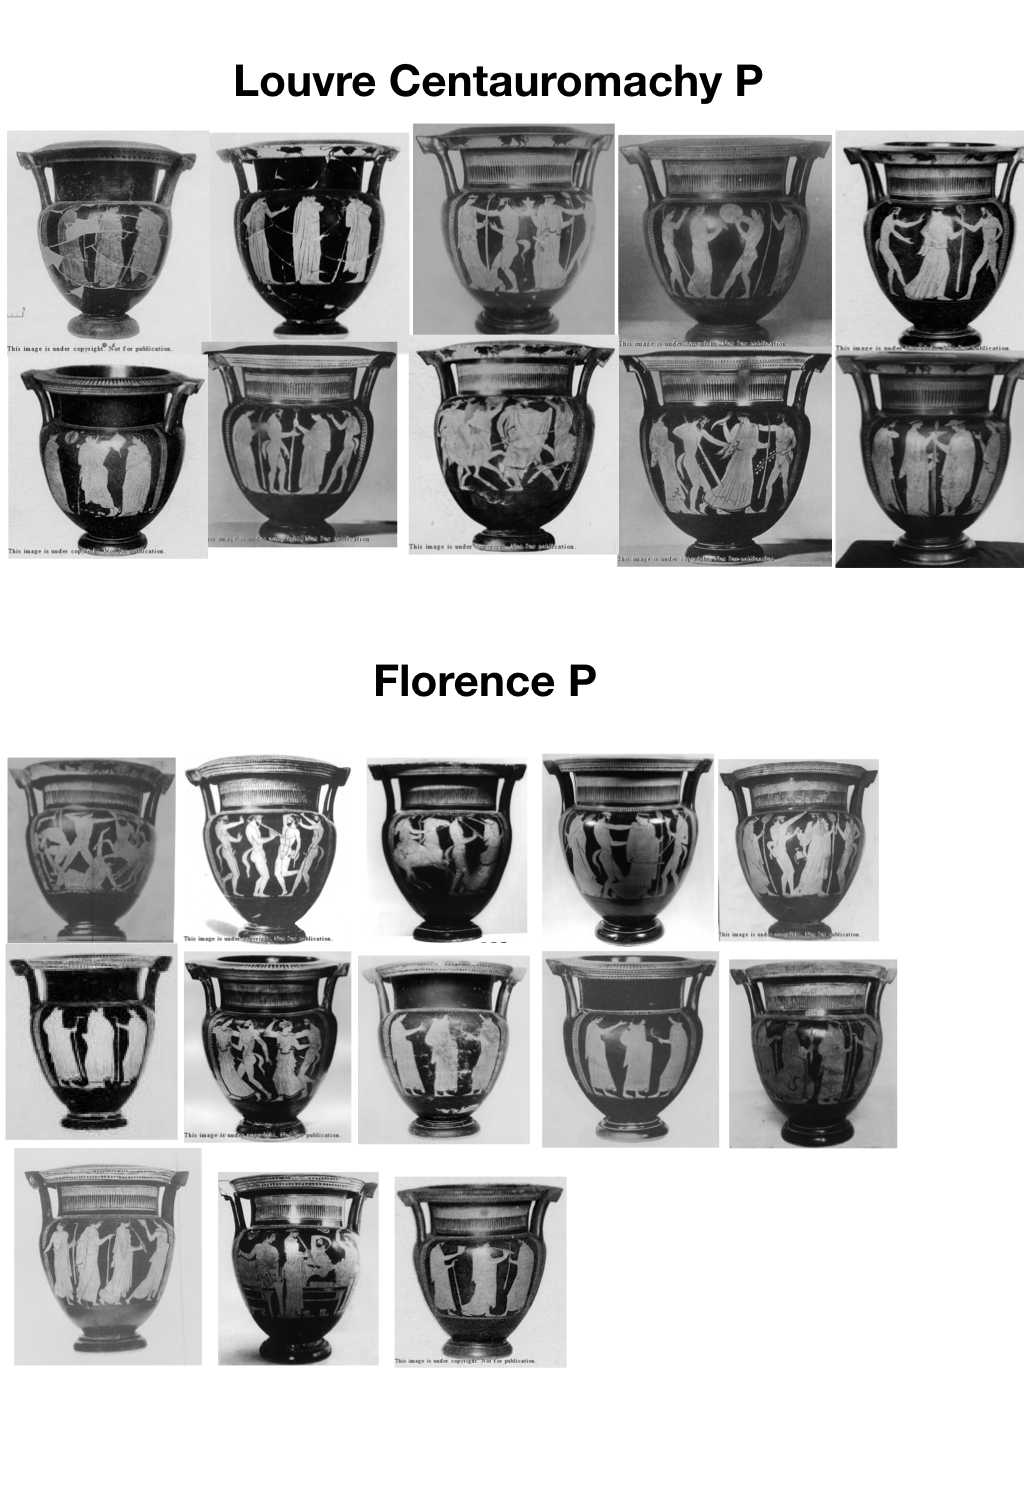
\includegraphics[width=8 cm]{colkrat}
 \caption{The vases made by two column krater painters from Athens. Are the Florence P vases, on average, slimmer than the Louvre Cent. P's vases?}
 \label{fig: krater}
\end{figure}

Thomas Mannack suggests that these particular painters are second-division and that we should focus on the Berlin painter and others like him.  We can, or we test the hypothesis with all the available data.

NOTE previous work: \cite{Ryan2009} asks just this question for Greek vases attributed to the Princeton Painter.  He extracts the outlines of 29  belly amphorae manually from CVA images, and then describes the shapes using various extracted features, among them series based on Hough and discrete Radon transforms. Using a Linear Discriminant Analysis he then asks if he can classify the vases attributed to Exekias, Andokides, Amasis and the Princeton Painter. In general he can. That he can do so for Exekias, Andokides and Amasis is not surprising: they signed their vases.  That he can do so for the Princeton potter is surprising, since it was claimed by Bloesch in \cite{Chamay1987} that no two vases in the Princeton Painter's corpus were made by the same potter. 

\item \textbf{within-potter variance}  If we knew how accurately a given potter threw vases at any given time we could estimate, perhaps, how many potters are active in Athens at any given time; or parameters for an evolutionary model. We could, for example, study the vases found in the Pointe Lequin 1A wreck: 1700 Ionian B2 cups probably made in a single workshop in Sicily.  The wreck was found off Marseille and the cups are at an institute in France. We'd have to go there and photograph them.   Nikosthenic vases would give the same thing (see below). And so, too, would replicate vases from modern workshops.


\end{enumerate}

\subsection*{The evolution of vase shape}
This section is concerned with understanding the evolutionary relationships among vases.  This is the general problem of phylogeny and can be investigated at several scales:  globally and for specific vase shapes or even sub-shapes
\begin{enumerate}

\item \textbf{Trends.}  \textcite{Bloesch1940, Bloesch1951}  claimed that, in the late Archaic period, ``the development of Greek vase-shapes follows a regular course, from heavy and plump forms to slender and more elegant.'' This pattern appears to be interrupted in -510 when, according to Bloesch, new shapes were invented and long-established forms modified. ``The vases become more full-bodied, with a more coherent outline''.  The claim is that this  trend can be seen in even in vases attributed to particular painters such as  Andokides and  Exekias \parencite{Mackay2010}.

As given in \textcite{Bloesch1951}, these claims are based entirely on qualitative data:  pictures of vases, but no numbers, not even height-width ratios.  We could test this claim.  The Beazley has dates for Red-Figure and Black-Figure Athenian vases $\pm$ 25 years, and Thomas Mannack says that they can be trusted, though perhaps they'd need some checking. We could certainly devise some metrics that capture ``heavy'', ``plump'' and  ``full-bodied'' v. ``slender'', ``elegant'' --- though I don't know what ``a more coherent outline'' looks like. 

Ideally, we'd be able to look for trends beyond Athenian BF and RF vases, for example, into earlier Geometric, Protogeometric etc, or later into Hellenistic vases. But to do that we'd need dates and, although dates (with wider ranges than Athenian classical) are available in the CVA, we'd have to enter them ourselves manually and curate them, and that's a lot of work which is best deferred. 

\item \textbf{Phylogeny.} Perhaps the most interesting thing we might do is build a phylogeny.  To do this I think we need to take the contours of each of our vases and, in some fashion, re-describe them in terms of a series of continuous characters.  I am unclear how to do this, but can imagine three ways, all of them vague: 
\begin{enumerate}
    \item the contours are described on an x-y coordinate grid. For any vase, each x value is an initial character, and the corresponding y value is its value. You then reduce the dimensionality by PCA, and the principal components are your final characters. 
    \item extract higher-level features from each of the contours. I am vague as to what these are, but I believe that many have been developed (e.g., the Hough and discrete Radon transforms used by \cite{Ryan2009}): these shape-features, then, are your final characters.
    \item something like (1) but then based on a dimensionality reduction method that emerges from Arianna's and Stephen's math. That's even vaguer.
\end{enumerate}

It's unclear whether we'd build a phylogeny of individual vases or of groups of vases. If the latter --- how do you group them?  By the traditional typology? Or by some cluster analysis based on their shapes?  Regardless of which you choose, or how, exactly, you get your continuous characters, what you do with the data is relatively clear.  That's because reconstruction of phylogenies from continuous characters has recently become of interest and there is a smallish literature devoted to model-based methods for doing so. \cite{Parins2017}, for example, estimated the phylogenies of a set of simulated phylogenies, upon which a set of continuous characters had been allowed to evolve.  She did this using RevBayes \parencite{Huelsenbeck2016}, provides scripts, and found that she could retrieve the true phylogenies quite well. There are other models that you can use as well such as Ornstien-Uhlenbeck (OU) and L\'{e}vy processes. Under BM, evolution is described as a random walk, with phenotypic change being normally distributed with a mean displacement of zero, and variance. OU models expand upon this by introducing terms producing a stabilizing force which stabilizes movement around an optimal trait value, while L\'{e}vy processes contain terms producing saltational jumps in character space, interspersed either by BM diffusion or stasis.  I suppose you can do model selection.

A classical phylogeny does not identify ancestors, but rather relatives. That is, it treats all taxa --- vases --- as contemporaneous. That is not ridiculous since it is possible that a new shape is inspired by an old one although \emph{a priori} we'd expect vases of nearby dates  (of a given class) to be  more closely related than those of distant dates.  However, given the sheer number of vases in our data set it seems possible that it actually contains real ancestors.  For example, the Athenian ``Nikosthenic amphora'', discussed below, is thought to be a direct descendant --- imitation --- of an Etruscan \emph{bucchero} shape. 

Of course, this is an issue in paleontology as well. Recently, new Bayesian phylogenetic methods have been introduced to account for the possibility that some of the sampled taxa are the ancestors of others.  \cite{Gavryushkina2014} develope a method to infer such ``sampled ancestor trees''.  The method requires date information for taxa, is implemented in the BEAST2 package, and can be used for morphological characters, as in this study on penguins \parencite{Drummond2016}. I don't know if continuous traits are supported by BEAST2 (some Google comments in 2018 suggest not).   Identifying ancestor-descendant relationships requires dates.  Getting dates for every single non-Athenian RF and BF vase would be difficult, but we could certainly get dates for classes of vases.  We know, for example, that Geometric vases are  -900 -- -700, and the Orientalizing style in Corinth and Athens -725 -- -625. So that would already significantly constrain the model.

All these methods are complicated.  There are innumerable choices of priors and generative models that have to be made, and the output is difficult to interpret.  We'd need to collaborate with an expert. The ``sampled ancestor trees'' method comes out of Auckland, so perhaps some Kiwi bonding might be in order. 

\item \textbf{The origins of Athenian ``orphans''.} Such a phylogeny could be used to investigate the origins of particular classes of vases.  For example, it is said that a bunch of shapes, among them some cup types and the stamnos, the pelike, and the kalpis  appear suddenly in Athens in the 6th C, perhaps around -510 \parencite{Bloesch1951}. Insofar that these shapes do not appear to be descended from any extant Athenian vases we can call them ``orphans''.  There are claims that at least some orphan shapes were borrowed from Corinth, an earlier vase-making centre.  If so, a phylogeny should show that the Athenian orphans are sister taxa to some Corithian shapes. Of course, we do not need a gobal vase phylogeny to test such hypotheses, for we could do test them on a case-by-case basis, but a phylogeny would be neater. 

\item \textbf{Nikosthenic vases.} There are certain classes of vases that are said to imitate others. For example, in Athens there are vases made by one Nikosthenes (he actually signed them for once) that imitate Etruscan (Central Italian, red-figure) precisely so that he could sell them on the Etruscan market. I don't know if these are in the Beazley database, but we could pull together such a collection of vases and ask if they really are that similar.  This, too, could be tested in the context of a global phylogeny. To do this we'd need images of Etruscan \emph{bucchero} which I do not think is well represented in the Beazley. But I have a monograph that contains all we want in terms of detail and images \parencite{Tosto1999}.

\item \textbf{Material \emph{konai} and Ionian B2 cups.} There are certain kinds of vessels made in a stereotyped way all over the Greek world. Archaeologists use the term \emph{koinai} to speak of this shared Greek culture. The most obvious of these are Ionian B2 cups. These aren't high-class painted cups; they're more humble, so there aren't many I think in the Beazley. They're Archaic, --600 to --540 or so. They were originally made in East Greece (Ionia) but then all over the place, e.g., Sicily.  There are loads of them, for example, the Pointe Lequin 1A wreck but, as noted above, we'd have to go there and photograph them and then get similar photos for another bunch of them made somewhere else. So we'd be asking: how similar \emph{are} these ``Ionian B2 cups'' made in different places? 
\item But there must be other examples of interesting evolutionary ideas to be tested. 
\end{enumerate}

\clearpage

\section*{Discussion}
\begin{enumerate}
\item The utility of the technique.  Its general applicability, particularly to large numbers of coarse-ware (transport amphorae etc). 
\item Maybe we even want to propose a controlled ontology for vase shape. (maybe this is too ambitious). It appears to be rather uncontrolled (see Cook). I am struck that it's not very good. This would require the authority of some vase experts. It's almost certainly for another paper, if that, but could be alluded. 
%\item The main limitation to the large-scale study of vase shape evolution is the state of the Beazley data.  It needs to be curated and checked by experts and modern dates put in. The whole vase ontology needs to be revised.
\item Future. Study the evolution of vases, build a phylogeny, study rates of evolution, look for revolutions, study selective forces etc --- all that cultural evolution stuff. 

\end{enumerate}
\printbibliography
\clearpage

\end{document}

